\documentclass[border=4pt]{standalone}
\usepackage{amsmath,amssymb}
\usepackage{tikz}
\usetikzlibrary{arrows.meta,decorations.pathreplacing,calc}
\begin{document}
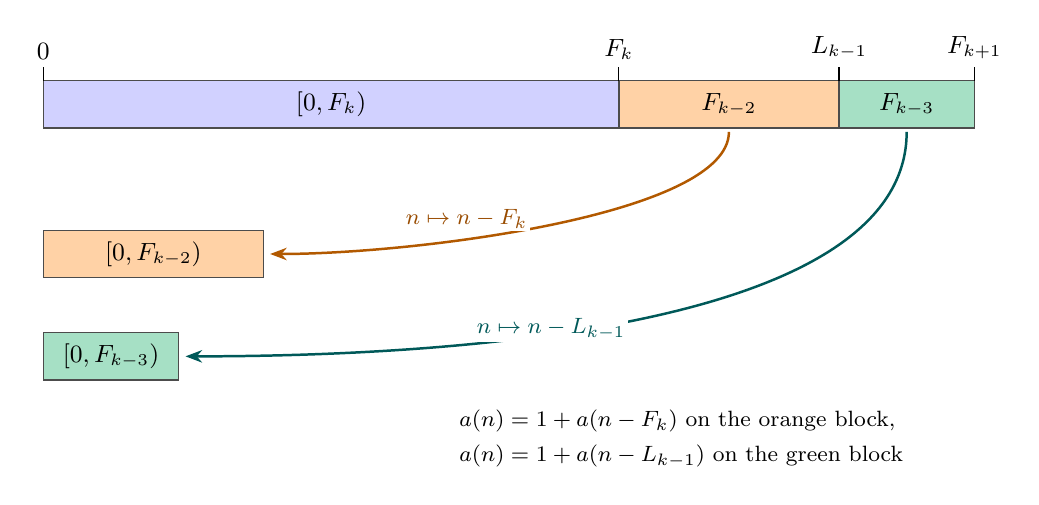
\begin{tikzpicture}[x=0.215cm,y=1cm,
  lab/.style={font=\small},
  note/.style={font=\footnotesize,align=center},
  blk/.style={draw=black!70,line width=0.5pt}]
  % k = 9: F_9 = 34, L_8 = 47, F_10 = 55, F_7 = 13, F_6 = 8
  % top bar [0, F_{k+1})
  \fill[blue!18] (0,0) rectangle (34,0.6);
  \fill[orange!35] (34,0) rectangle (47,0.6);
  \fill[green!30!teal!35] (47,0) rectangle (55,0.6);
  \draw[blk] (0,0) rectangle (55,0.6);
  \draw[blk] (34,0) -- (34,0.6) (47,0) -- (47,0.6);
  \node[lab] at (17,0.3) {$[0,F_k)$};
  \node[lab] at (40.5,0.3) {$F_{k-2}$};
  \node[lab] at (51,0.3) {$F_{k-3}$};
  \foreach \x/\t in {0/0,34/F_k,47/L_{k-1},55/F_{k+1}} {
    \draw (\x,0.6) -- (\x,0.78);
    \node[lab,above] at (\x,0.75) {$\t$};
  }
  % bottom copies
  \fill[orange!35] (0,-1.9) rectangle (13,-1.3);
  \draw[blk] (0,-1.9) rectangle (13,-1.3);
  \node[lab] at (6.5,-1.6) {$[0,F_{k-2})$};
  \fill[green!30!teal!35] (0,-3.2) rectangle (8,-2.6);
  \draw[blk] (0,-3.2) rectangle (8,-2.6);
  \node[lab] at (4,-2.9) {$[0,F_{k-3})$};
  % arrows
  \draw[-{Stealth[length=6pt]},orange!70!black,line width=0.9pt]
     (40.5,-0.05) .. controls (40.5,-1.1) and (22,-1.6) .. (13.4,-1.6);
  \node[note,orange!60!black,fill=white,inner sep=1pt] at (25,-1.15) {$n\mapsto n-F_k$};
  \draw[-{Stealth[length=6pt]},teal!70!black,line width=0.9pt]
     (51,-0.05) .. controls (51,-2.5) and (25,-2.9) .. (8.4,-2.9);
  \node[note,teal!70!black,fill=white,inner sep=1pt] at (30,-2.55) {$n\mapsto n-L_{k-1}$};
  \node[note,anchor=west,align=left] at (24,-3.95) {$a(n)=1+a(n-F_k)$ on the orange block,\\[3pt] $a(n)=1+a(n-L_{k-1})$ on the green block};
\end{tikzpicture}
\end{document}
